\section{Rubin Observatory Commissioning}
\label{sec:commissioning}

\subsection{Commissioning Schedule}
\label{ssec:commissioning-schedule}

\TODO{red}{UPDATE following schedule workshop}

In December 2022, as a result of reoptimizing the sequence of integration activities, the Rubin Construction Project decided to install the LSST Science Camera (LSSTCam) on the telescope earlier in the assembly sequence than previously planned. 
As a consequence, no on-sky data will be taken with the Commissioning Camera (ComCam). 
This change in strategy will produce more early-commissioning data than would have been available with ComCam on a similar timeframe. 

\begin{figure}[htb]
\centering
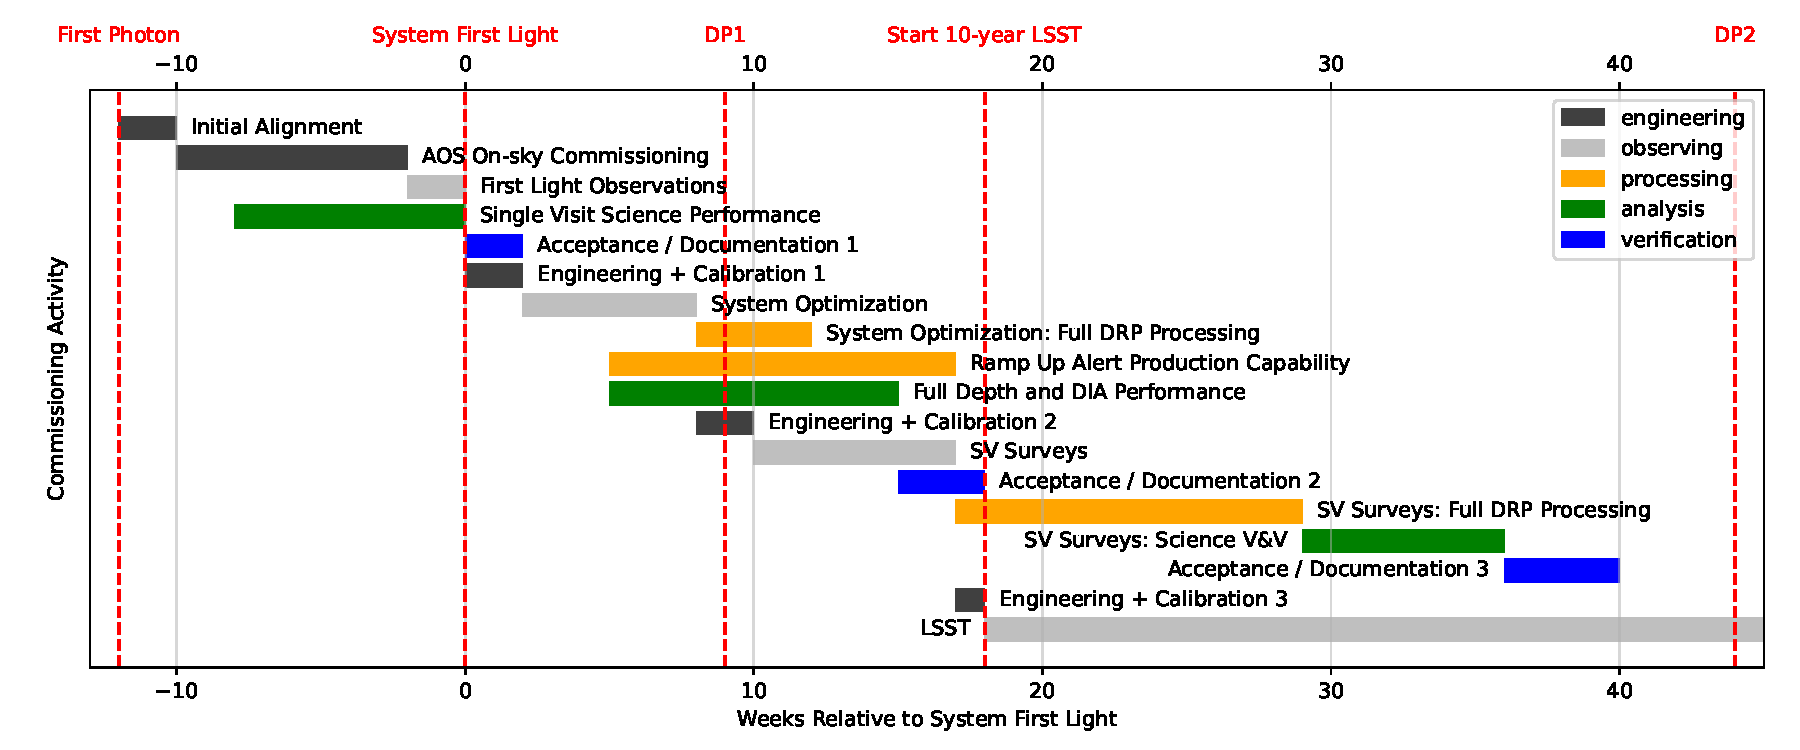
\includegraphics[width=0.95\linewidth]{figures/rubinobs_on-sky_commissioning_gantt.pdf}
\caption{Detailed schedule of commissioning activities relative to System First Light, as of December 2022.}
\label{fig:commissioning-gantt}
\end{figure}

Figure~\ref{fig:commissioning-gantt} shows the detailed schedule of commissioning activities relative to System First Light, as of December 2022.
System First Light is currently expected between October 2024 and February 2025 (\S~\ref{sec:timeline}), about 3 months after First Photon. 
The System First Light milestone marks the end of the the on-sky engineering phase and the start of the System Optimization and Science Validation phases. 
The total amount of science validation time currently planned is about 8 weeks.  
LSST data taking is expected to start about 4 months after System First Light.

As Rubin construction moves through the challenging phase of System Integration, Test and Commissioning, this schedule may change.

\subsection{Commissioning Observations}
\label{ssec:commissioning-observations}

Figure~\ref{fig:commissioning} shows the high level plan for the Rubin commissioning observations with the LSST Science Camera.
Commissioning data collection is planned to take place in phases.
Following the System First Light milestone, a set of observations designed to help optimize the system will be taken during the System Optimization phase before the Science Validation Surveys are carried out. 
The SV Surveys are designed to support scientific analyses that validate the system's performance, and allow Rubin to demonstrate operations readiness \citeds{SITCOMTN-005}.

\begin{figure}[htb]
\centering
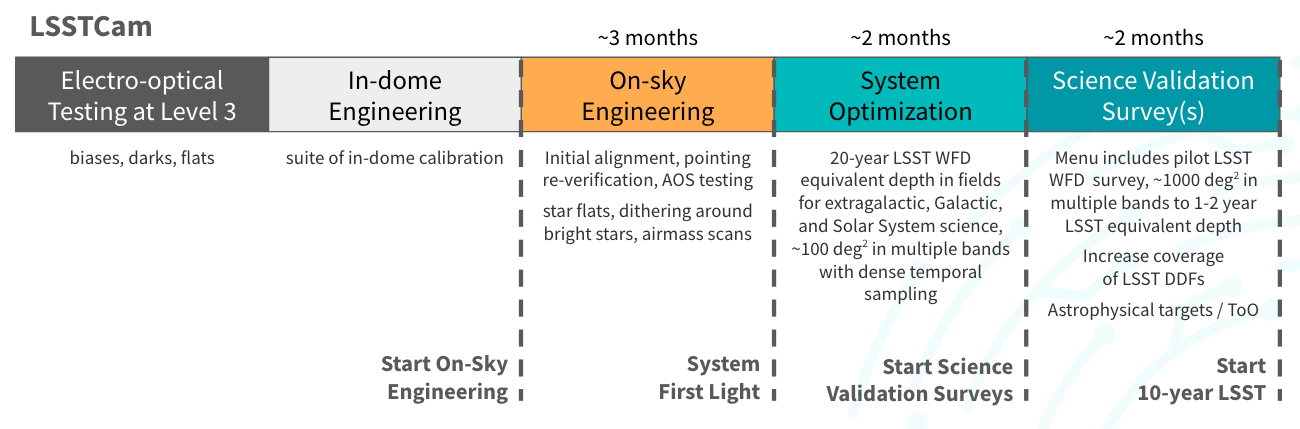
\includegraphics[width=0.95\linewidth]{figures/commissioning-plan}
\caption{Outline plan for the collection of commissioning data, as of December 2022.}
\label{fig:commissioning}
\end{figure}

Figure~\ref{fig:commissioning} also indicates a number of planned key components of the System Optimization and SV phases.
These include a LSST wide-fast-deep (WFD) 1-2 year equivalent depth ``pilot'' survey.
Field selection will be carried out by the Commissioning Team, taking into account a wide variety of constraints as well as a ``menu'' of science opportunities to which the LSST Science Community has contributed.
Details of the plans for commissioning observations will be made available as those plans converge, in this technote and other documents as cited.